\subsubsection{Vision Transformer Architecture}

The Vision Transformer (ViT) architecture comprises the following components:

\paragraph{Patch Embedding:}
The process begins by dividing the input image into non-overlapping patches. Each patch is then transformed into an embedding through a linear projection. These embeddings are further enhanced with positional encodings to provide information about the patch's position in the image.

\begin{figure}[htbp]
    \centering
    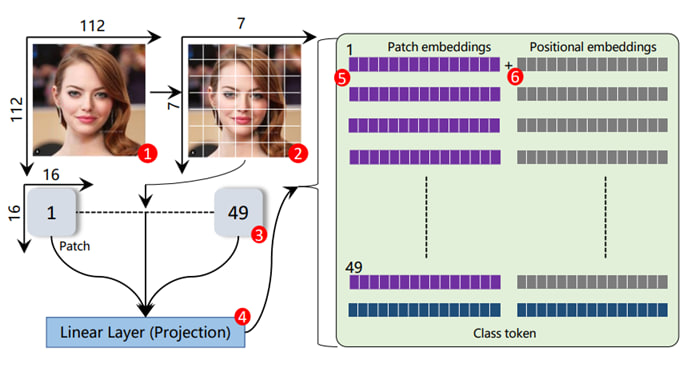
\includegraphics[width=6in]{img/patchembedding.jpg}
    \caption{Patch Embedding}
\end{figure}

\paragraph{Transformer Encoder:}
The patch embeddings are then processed through a stack of transformer encoder layers. Each of these layers consists of two main components: multi-head self-attention and feedforward neural networks.

\begin{enumerate}
    \item \textbf{Multi-head self-attention:} This mechanism allows the model to consider relationships between different patches, both locally and globally. It assigns different attention weights to different patches based on their relevance to each other, enabling the model to capture long-range dependencies and relationships within the image. \\
          \\
          \noindent \textbf{Standard qkv Self-Attention (SA)}:
          For an input sequence $z \in \mathbf{R}^{N \times D}$ (with $N$ elements, each having a $D$-dimensional feature vector), we compute a weighted sum over all values $v$ in the sequence. The attention weights $A_{ij}$ are determined based on the similarity between elements of the sequence and their corresponding query $q_i$ and key $k_j$ representations.
          \[
              [q, k, v] = zU_{qkv}, \quad U_{qkv} \in \mathbf{R}^{D \times 3Dh}
          \]
          \[
              A = \text{softmax}\left(\frac{qk^T}{\sqrt{Dh}}\right), \quad A \in \mathbf{R}^{N \times N}
          \]
          \[
              \text{SA}(z) = Av
          \]

          \textbf{Multihead Self-Attention (MSA)}:
          MSA extends SA by running $k$ self-attention operations (heads) in parallel and then concatenating their outputs. To ensure consistent computation and parameter complexity, the dimension $Dh$ (from Eq. 5) is usually set to $D/k$.
          \[
              \text{MSA}(z) = [SA_1(z); SA_2(z); \ldots ; SA_k(z)], \quad U_{msa} \in \mathbf{R}^{k \cdot Dh \times D}
          \]

    \item \textbf{Feedforward neural networks:} After the attention mechanism, the data passes through feedforward neural networks, which process and transform the information further, helping the model learn intricate features and patterns in the image data.
\end{enumerate}

\begin{figure}[htbp]
    \centering
    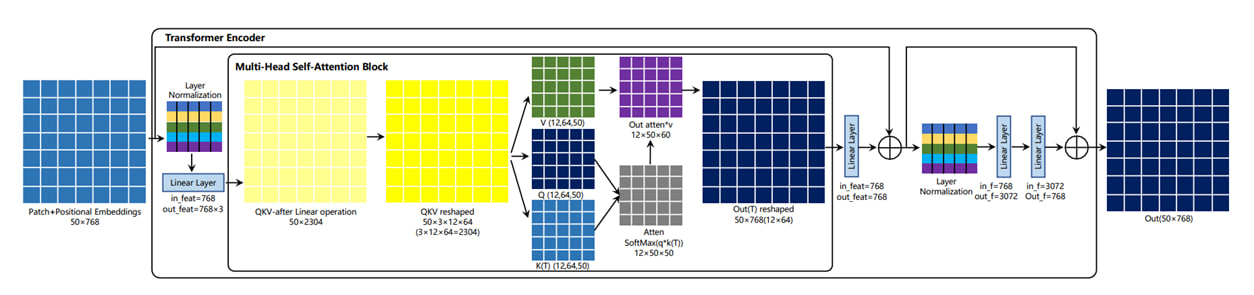
\includegraphics[width=6in]{img/encoderdetails.jpg}
    \caption{Transformer Encoder}
\end{figure}

\paragraph{Classification Head:}
At the top of the architecture, there's a classification head that takes the transformed embeddings and predicts whether an image is real or manipulated, based on the features and patterns the model has learned.

\begin{figure}[htbp]
    \centering
    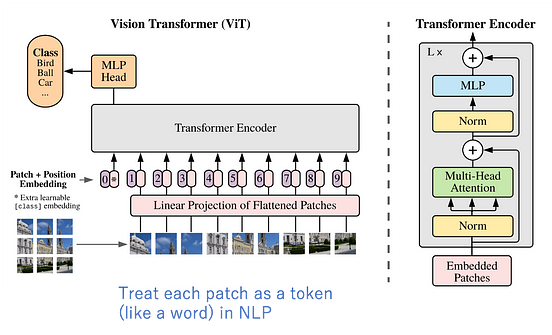
\includegraphics[width=6in]{img/visiontransformer.png}
    \caption{Vision Transformer Architecture}
\end{figure}

\newpage
